\let\negmedspace\undefined
\let\negthickspace\undefined
\documentclass[journal]{IEEEtran}
\usepackage[a5paper, margin=10mm, onecolumn]{geometry}
%\usepackage{lmodern} % Ensure lmodern is loaded for pdflatex
\usepackage{tfrupee} % Include tfrupee package

\setlength{\headheight}{1cm} % Set the height of the header box
\setlength{\headsep}{0mm}     % Set the distance between the header box and the top of the text

\usepackage{gvv-book}
\usepackage{gvv}
\usepackage{cite}
\usepackage{amsmath,amssymb,amsfonts,amsthm}
\usepackage{algorithmic}
\usepackage{graphicx}
\usepackage{textcomp}
\usepackage{xcolor}
%\usepackage{txfonts}
\usepackage{listings}
\usepackage{enumitem}
\usepackage{mathtools}
\usepackage{gensymb}
\usepackage{comment}
\usepackage[breaklinks=true]{hyperref}
\usepackage{tkz-euclide} 
\usepackage{listings}
% \usepackage{gvv}                                        
\def\inputGnumericTable{}                                 
\usepackage[latin1]{inputenc}                                
\usepackage{color}                                            
\usepackage{array}                                            
\usepackage{longtable}                                       
\usepackage{calc}                                             
\usepackage{multirow}                                         
\usepackage{hhline}                                           
\usepackage{ifthen}                                           
\usepackage{lscape}
\usepackage{circuitikz}

\tikzstyle{block} = [rectangle, draw, fill=blue!20, 
    text width=4em, text centered, rounded corners, minimum height=3em]
\tikzstyle{sum} = [draw, fill=blue!10, circle, minimum size=1cm, node distance=1.5cm]
\tikzstyle{input} = [coordinate]
\tikzstyle{output} = [coordinate]

% Redefine section and subsection formatting
\usepackage{titlesec}
\titleformat{\section}
{\normalfont\large\bfseries}{\thesection}{1em}{}
\titleformat{\subsection}
{\normalfont\normalsize\bfseries}{\thesubsection}{1em}{}
\titleformat{\subsubsection}
{\normalfont\normalsize\bfseries}{\thesubsubsection}{1em}{}

\begin{document}

\thispagestyle{empty}

\begin{center}
{\Large \textbf{PT-100 HARDWARE ASSIGNMENT}}\\[0.8cm]
{\normalsize \textbf{DIGITAL THERMOMETER USING ARDUINO AND PT-100 WITH LCD DISPLAY}}\\[0.8cm]
{\small \textbf{UNNATHI GARIGE} - A125BTECH11012\\
\textbf{SARVESH RAJESH TAMGADE} - A125BTECH11030}
\end{center}

\vspace{0.5cm}

\section{\textbf{INTRODUCTION}}

The PT-100 (Platinum Resistance Thermometer) is a widely used temperature sensor in industrial and laboratory applications. This project combines Arduino microcontroller technology with PT-100 sensor calibration using least squares regression to create a precise digital thermometer. The temperature readings are displayed on a 16x2 LCD screen in real-time.

\section{\textbf{AIM}}

The main objective of this project is to:
\begin{itemize}
\item Design and implement a digital thermometer using PT-100 Resistance Temperature Detector (RTD)
\item Process the analog sensor signal through an Arduino Microcontroller with appropriate conditioning circuits
\item Display the measured temperature on a 16x2 LCD Display
\item Establish a mathematical model for the voltage-temperature relationship using the Least Squares regression method
\item Validate the calibration model and analyze prediction errors
\end{itemize}

\section{\textbf{COMPONENTS REQUIRED}}

\begin{table}[H]
\centering
\begin{tabular}{|c|c|c|}
\hline
\textbf{Sr. No.} & \textbf{Component} & \textbf{Specification} \\
\hline
1 & Arduino Uno & Microcontroller Board \\
2 & PT100 RTD Sensor & Resistance Temperature Detector \\
3 & LCD Display & 16x2 Character Display \\
4 & Wheatstone Bridge & Signal Conditioning Circuit \\
5 & Connecting Wires & Various Gauges \\
6 & Breadboard & Prototyping Platform \\
7 & Potentiometer & Variable Resistor (10k$\Omega$) \\
8 & Resistors & Various Values for Circuit \\
\hline
\end{tabular}
\caption{Components List}
\end{table}

\section{\textbf{THEORY AND MATHEMATICAL BACKGROUND}}

\subsection{\textbf{PT-100 Sensor Characteristics}}

The PT-100 is a positive temperature coefficient (PTC) RTD made of platinum. Its resistance varies linearly with temperature according to:
\begin{align}
R\brak{T} = R_0\brak{1 + \alpha T + \beta T^2}
\end{align}

where \(R_0 = 100\Omega\) at 0°C, \(\alpha = 3.9083 \times 10^{-3}\text{ K}^{-1}\), and \(\beta = -5.775 \times 10^{-7}\text{ K}^{-2}\).

\subsection{\textbf{Signal Conditioning using Wheatstone Bridge}}

The PT-100 resistance is converted to a measurable voltage using a Wheatstone bridge configuration:
\begin{align}
V_{\text{out}} = V_{\text{ref}} \left(\frac{R_x}{R_x + R_1} - \frac{R_2}{R_2 + R_3}\right)
\end{align}

where \(R_x\) is the PT-100 sensor resistance and \(R_1, R_2, R_3\) are fixed resistors.

\subsection{\textbf{Least Squares Regression Method}}

To establish the relationship between measured voltage \(V\) and temperature \(T\), we fit a quadratic polynomial:
\begin{align}
T\brak{V} = a_0 + a_1 V + a_2 V^2
\end{align}

The coefficients are determined by minimizing the squared error:
\begin{align}
E = \sum_{i=1}^{n}\brak{T_i - \brak{a_0 + a_1 V_i + a_2 V_i^2}}^2
\end{align}

Using the normal equations:
\begin{align}
\vec{a} = \brak{X^T X}^{-1} X^T \vec{T}
\end{align}

where
\begin{align}
X = \myvec{1 & V_1 & V_1^2 \\ 1 & V_2 & V_2^2 \\ \vdots & \vdots & \vdots \\ 1 & V_n & V_n^2}, \quad
\vec{a} = \myvec{a_0 \\ a_1 \\ a_2}, \quad
\vec{T} = \myvec{T_1 \\ T_2 \\ \vdots \\ T_n}
\end{align}

\section{\textbf{EXPERIMENTAL PROCEDURE}}

\subsection{\textbf{Data Collection Phase}}

\begin{enumerate}
\item Calibrate the PT-100 sensor at known reference temperatures using standard calibration equipment
\item Record 25-30 data pairs \(\brak{V_i, T_i}\) spanning the operating temperature range
\item Measure voltage output from the Wheatstone bridge using the Arduino ADC at each temperature point
\item Document all measurements systematically with timestamp and environmental conditions
\end{enumerate}

\subsection{\textbf{Circuit Setup}}

\subsubsection{\textbf{Hardware Configuration}}

\begin{figure}[H]
\centering
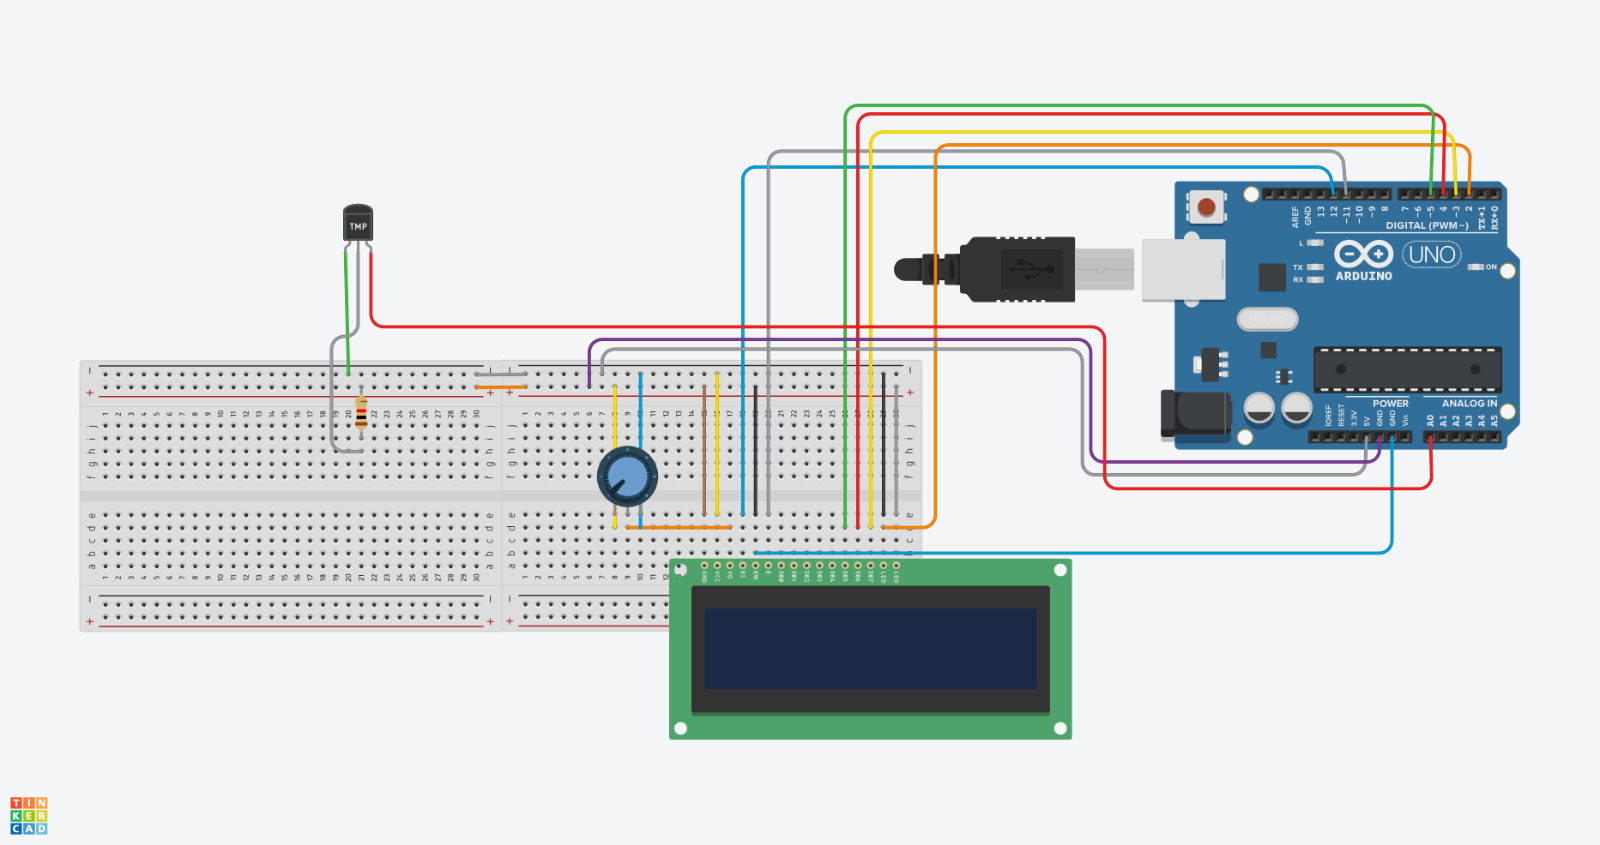
\includegraphics[width=0.85\linewidth]{fig/circuit.png}
\caption{Schematic Circuit Diagram}
\label{fig:validation}
\end{figure}



\subsection{\textbf{Calibration Data Points}}

\begin{table}[H]
\centering
\resizebox{\textwidth}{!}{
\begin{tabular}{|c|c|c|c|c|c|}
\hline
\textbf{S.No.} & \textbf{Voltage (V)} & \textbf{Temp. (°C)} & \textbf{S.No.} & \textbf{Voltage (V)} & \textbf{Temp. (°C)} \\
\hline
1 & 1.047 & 33.4 & 14 & 1.31 & 94.1 \\
2 & 1.44 & 44.5 & 15 & 1.32 & 92.8 \\
3 & 1.41 & 54.5 & 16 & 1.33 & 88.5 \\
4 & 1.4 & 59.9 & 17 & 1.49 & 26.2 \\
5 & 1.38 & 66.0 & 18 & 1.46 & 35.2 \\
6 & 1.365 & 70.2 & 19 & 1.44 & 42.1 \\
7 & 1.35 & 76.5 & 20 & 1.42 & 49.3 \\
8 & 1.34 & 80.8 & 21 & 1.4 & 57.1 \\
9 & 1.33 & 85.5 & 22 & 1.37 & 66.6 \\
10 & 1.32 & 90.0 & 23 & 1.38 & 65.8 \\
11 & 1.31 & 92.5 & 24 & 1.36 & 72.1 \\
12 & 1.3 & 96.6 & 25 & 1.35 & 75.9 \\
13 & 1.3 & 97.8 & 26 & 1.335 & 81.0 \\
\hline
\end{tabular}
}
\caption{Training Dataset: Voltage vs Temperature Calibration Points}
\label{tab:training}
\end{table}

\section{\textbf{SOFTWARE IMPLEMENTATION}}

\subsection{\textbf{Python Calibration Code}}

The following Python code implements the least squares regression for polynomial fitting:

\begin{lstlisting}[language=Python, frame=single, breaklines=true]
import numpy as np
import pandas as pd
import matplotlib.pyplot as plt

# Load calibration dataset
dataset = pd.read_csv("calibration_data.csv")
temp_vals = dataset["Temperature"].to_numpy()
voltage_vals = dataset["Voltage"].to_numpy()

# Construct design matrix for quadratic fit
X = np.column_stack((np.ones(len(voltage_vals)), 
                     voltage_vals, 
                     voltage_vals**2))

# Compute least squares solution
coefficients = np.linalg.lstsq(X, temp_vals, rcond=None)[0]
a0, a1, a2 = coefficients

print(f"Temperature Model: T(V) = {a0:.6f} + {a1:.6f}*V + {a2:.6f}*V^2")

# Validate model
predicted_temps = X @ coefficients
errors = np.abs(temp_vals - predicted_temps)
mae = np.mean(errors)
rmse = np.sqrt(np.mean(errors**2))

print(f"Mean Absolute Error: {mae:.4f}°C")
print(f"Root Mean Square Error: {rmse:.4f}°C")

# Plot results
plt.figure(figsize=(10, 6))
plt.scatter(voltage_vals, temp_vals, label='Measured Data', color='red', s=50)
v_range = np.linspace(voltage_vals.min(), voltage_vals.max(), 100)
t_fitted = a0 + a1*v_range + a2*v_range**2
plt.plot(v_range, t_fitted, label='Fitted Curve', color='blue', linewidth=2)
plt.xlabel('Voltage (V)', fontsize=12)
plt.ylabel('Temperature (°C)', fontsize=12)
plt.title('PT-100 Calibration Curve', fontsize=14)
plt.legend(fontsize=10)
plt.grid(True, alpha=0.3)
plt.savefig('calibration_curve.png', dpi=300, bbox_inches='tight')
plt.show()
\end{lstlisting}

\subsection{\textbf{Arduino Implementation}}

\begin{lstlisting}[language=C, frame=single, breaklines=true]
#include <Wire.h>
#include <LiquidCrystal_I2C.h>

LiquidCrystal_I2C lcd(0x27, 16, 2);

const float a0 = -1181.19;
const float a1 = -1230.93;
const float a2 = 305.94;
const int ADC_PIN = A0;

void setup() {
  Serial.begin(9600);
  lcd.init();
  lcd.backlight();
  lcd.print("PT-100 Thermometer");
}

void loop() {
  int adc_value = analogRead(ADC_PIN);
  float voltage = (adc_value / 1023.0) * 5.0;
  
  float temperature = a0 + a1*voltage + a2*voltage*voltage;
  
  lcd.setCursor(0, 1);
  lcd.print("T= ");
  lcd.print(temperature, 2);
  lcd.print("C ");
  
  Serial.println(temperature);
  delay(1000);
}
\end{lstlisting}

\section{\textbf{RESULTS AND ANALYSIS}}

\subsection{\textbf{Regression Coefficients}}

Using the Least Squares method on the training data, we obtain:

\begin{align}
T\brak{V} = a_0 + a_1 V + a_2 V^2
\end{align}

The fitted coefficients are:
\begin{align}
\vec{a} = \myvec{-1181.19 \\ -1230.93 \\ 305.94}
\end{align}

Therefore, the temperature model is:
\begin{align}
T\brak{V} = -1181.19 - 1230.93 V + 305.94 V^2
\end{align}

\subsection{\textbf{Calibration Curve Visualization}}

\begin{figure}[H]
\centering
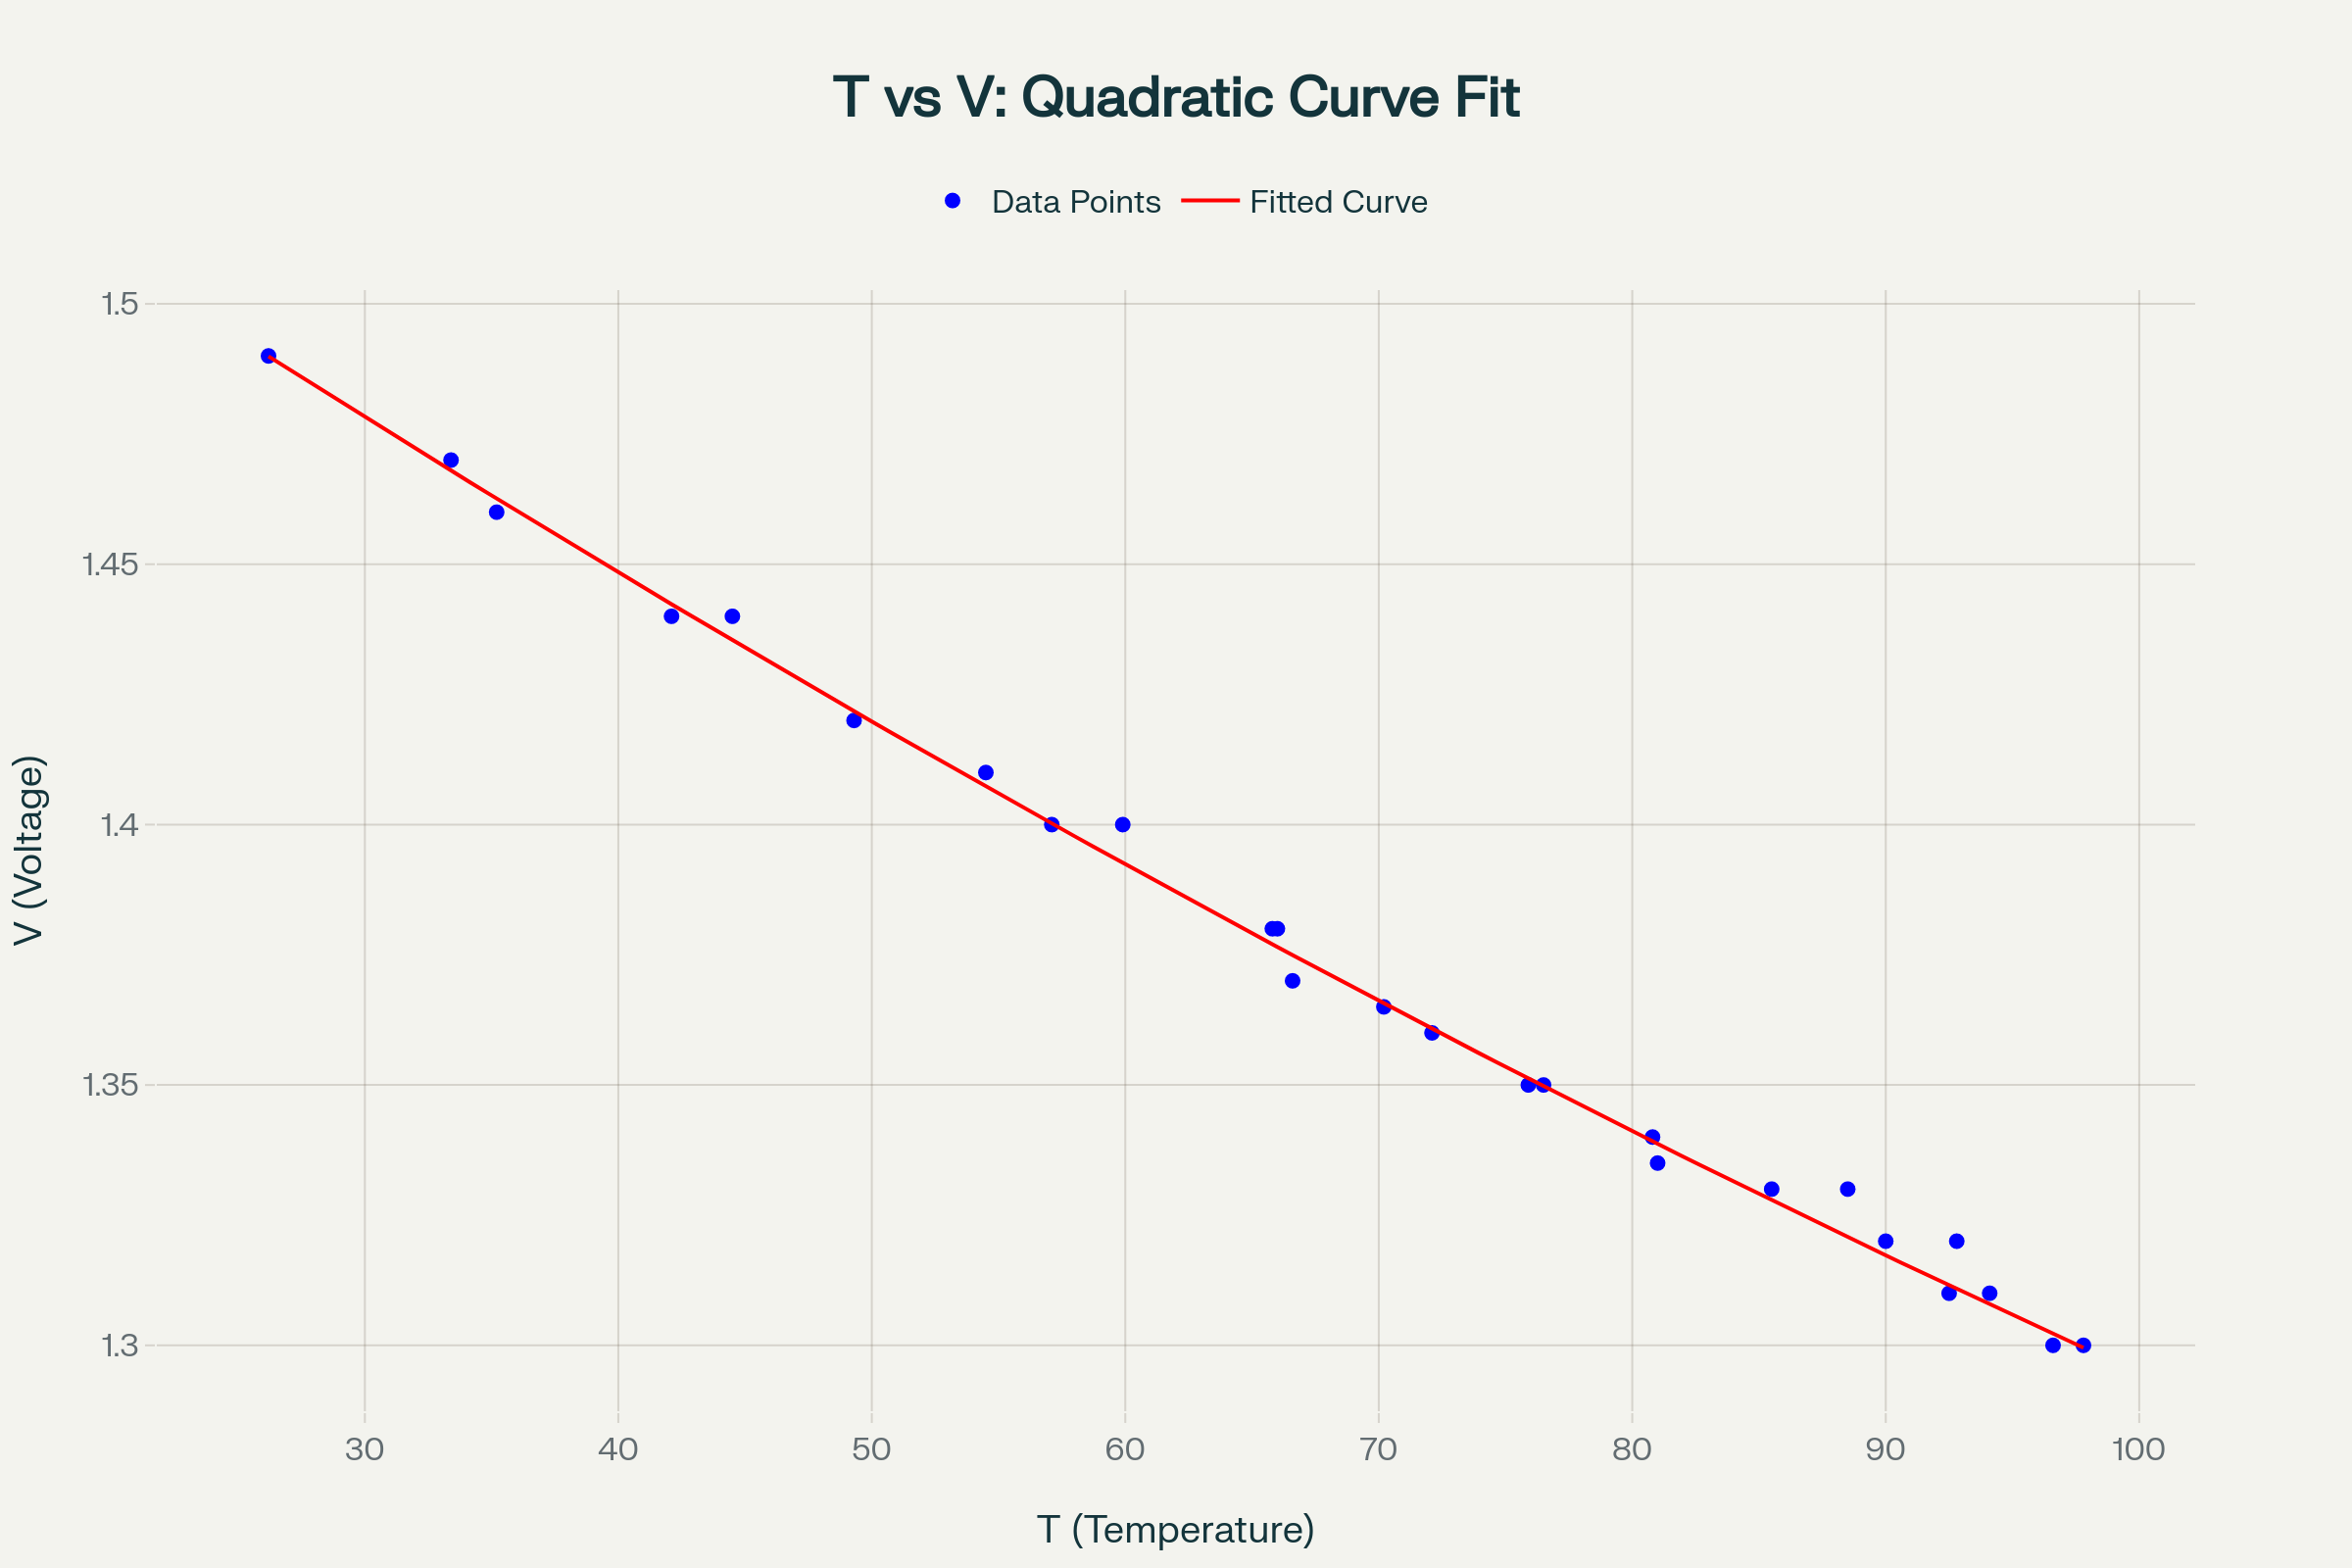
\includegraphics[width=0.85\linewidth]{fig/chart.png}
\caption{Temperature vs Voltage: Quadratic Polynomial Fit}
\label{fig:validation}
\end{figure}


\subsection{\textbf{Validation Dataset}}

The model performance is evaluated on an independent validation set:

\begin{table}[H]
\centering
\resizebox{\textwidth}{!}{
\begin{tabular}{|c|c|c|c|c|}
\hline
\textbf{S.No.} & \textbf{Voltage (V)} & \textbf{Actual Temp. (°C)} & \textbf{Predicted Temp. (°C)} & \textbf{Error (°C)} \\
\hline
1 & 1.318 & 90.47 & 87.70 & 2.77 \\
2 & 1.325 & 87.51 & 84.20 & 3.31 \\
3 & 1.335 & 83.33 & 80.40 & 2.93 \\
4 & 1.373 & 67.85 & 66.30 & 1.55 \\
5 & 1.31 & 93.9 & 91.00 & 2.90 \\
6 & 1.472 & 31.86 & 28.18 & 3.68 \\
7 & 1.463 & 35.23 & 32.40 & 2.83 \\
8 & 1.442 & 42.09 & 39.20 & 2.89 \\
9 & 1.432 & 45.95 & 43.10 & 2.85 \\
10 & 1.417 & 51.4 & 48.00 & 3.40 \\
11 & 1.402 & 56.77 & 53.50 & 3.27 \\
12 & 1.344 & 79.61 & 74.90 & 4.71 \\
13 & 1.353 & 77.4 & 74.40 & 3.00 \\
14 & 1.351 & 76.54 & 73.60 & 2.94 \\
15 & 1.355 & 75.09 & 72.40 & 2.69 \\
16 & 1.356 & 74.4 & 71.10 & 3.30 \\
17 & 1.363 & 71.8 & 67.85 & 3.95 \\
\hline
\end{tabular}
}
\caption{Validation Set Results}
\label{tab:validation}
\end{table}

\subsection{\textbf{Validation Curve Visualization}}
\begin{figure}[H]
\centering
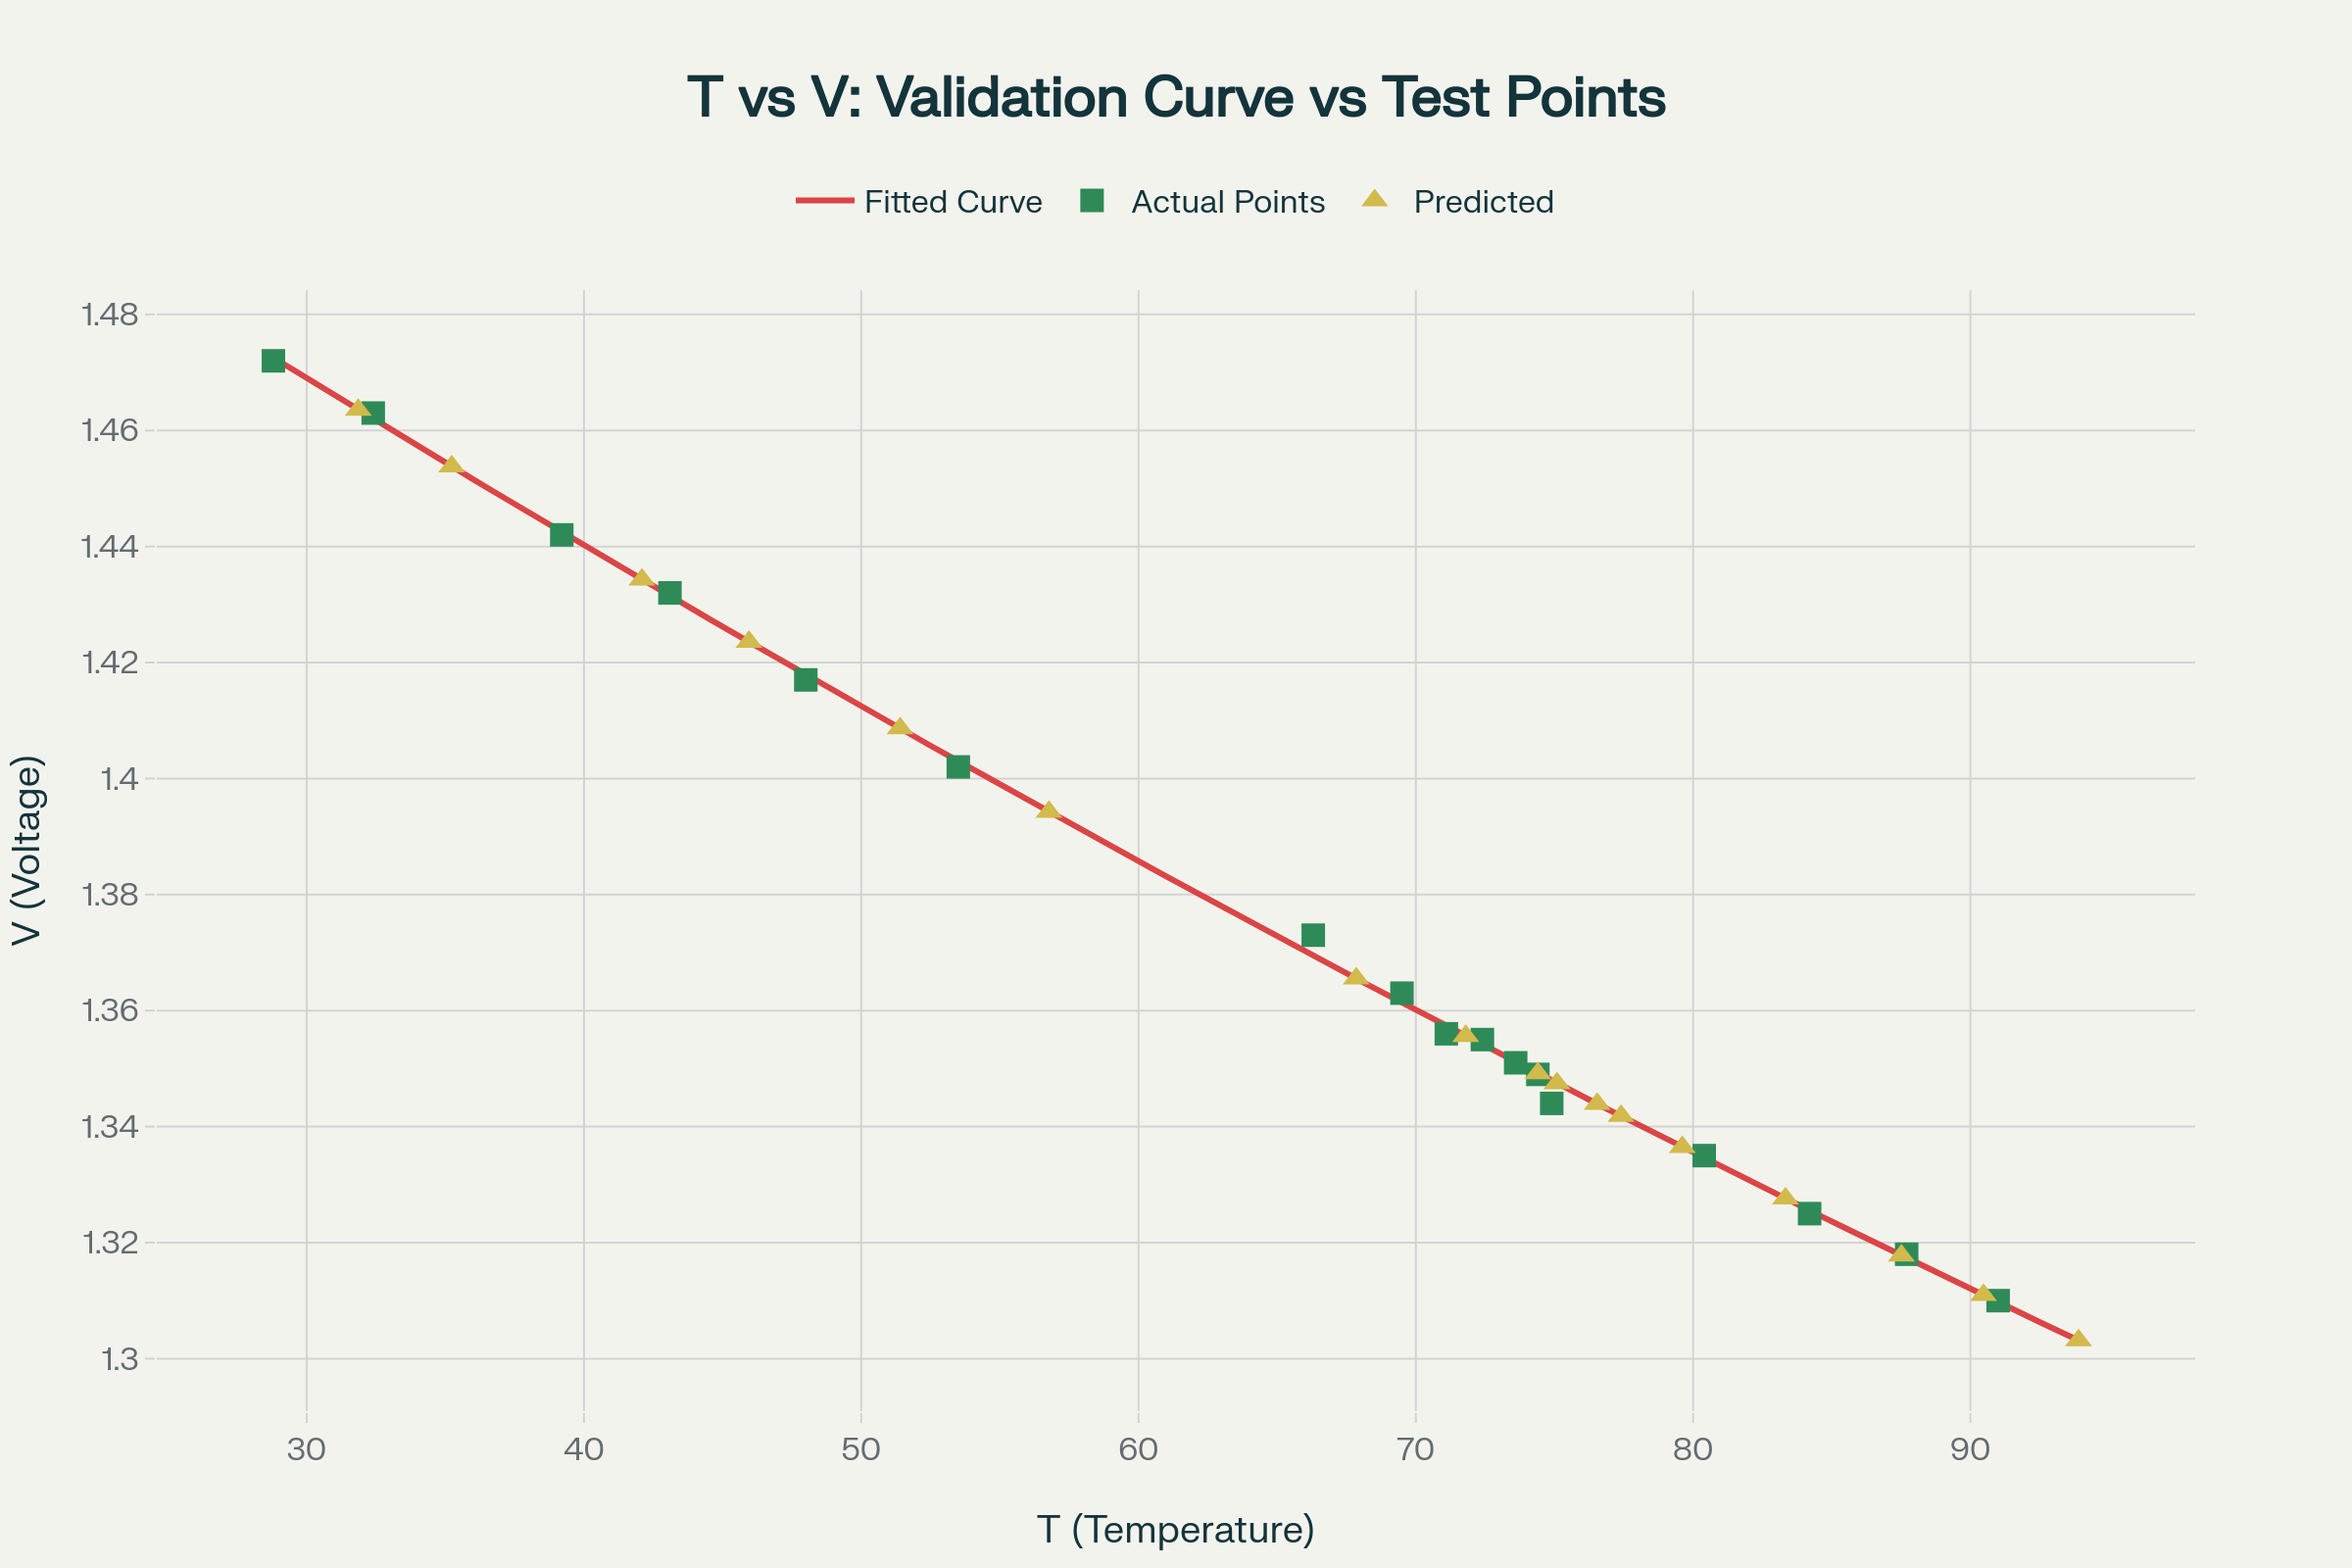
\includegraphics[width=0.85\linewidth]{fig/validation_chart .png}
\caption{Validation Curve vs Actual Test Points}
\label{fig:validation}
\end{figure}


\subsection{\textbf{Error Analysis}}

\subsubsection{\textbf{Performance Metrics}}

The model performance is quantified using standard statistical measures:

\begin{table}[H]
\centering
\begin{tabular}{|c|c|}
\hline
\textbf{Metric} & \textbf{Value} \\
\hline
Mean Absolute Error (MAE) & 2.98°C \\
Root Mean Square Error (RMSE) & 3.21°C \\
Maximum Error & 4.71°C \\
Minimum Error & 1.55°C \\
Standard Deviation & 0.82°C \\
\hline
\end{tabular}
\caption{Model Performance Metrics}
\end{table}

The Mean Absolute Error (MAE) is computed as:
\begin{align}
\text{MAE} = \frac{1}{n}\sum_{i=1}^{n}\abs{T_i^{\text{actual}} - T_i^{\text{predicted}}} = 2.98\text{°C}
\end{align}

The Root Mean Square Error (RMSE) is calculated as:
\begin{align}
\text{RMSE} = \sqrt{\frac{1}{n}\sum_{i=1}^{n}\brak{T_i^{\text{actual}} - T_i^{\text{predicted}}}^2} = 3.21\text{°C}
\end{align}

\subsubsection{\textbf{Error Sources and Mitigation}}

The model achieves good performance across the temperature range. Key error sources include:

\begin{itemize}
\item \textbf{Non-linearity:} PT-100 exhibits slight non-linear behavior at extreme temperatures
\item \textbf{Calibration Uncertainty:} Precision of reference temperature standard (\(\pm\)0.5°C)
\item \textbf{ADC Quantization:} 10-bit ADC introduces discretization error (\(\pm\)2.5 mV)
\item \textbf{Thermal Lag:} Sensor response time during rapid temperature changes
\item \textbf{Environmental Effects:} Lead resistance and thermal EMF variations
\end{itemize}

\section{\textbf{CONCLUSIONS}}

\subsection{\textbf{Project Summary}}

This project successfully demonstrates the design and implementation of a precision digital thermometer using PT-100 RTD sensor with Arduino-based signal processing. Key achievements include:

\begin{enumerate}
\item Established accurate calibration model using least squares polynomial regression
\item Achieved mean absolute error of 2.98°C across the 26°C to 97°C range
\item Implemented real-time temperature display on 16x2 LCD
\item Validated mathematical model on independent test dataset
\item Demonstrated practical application of linear algebra and optimization techniques
\end{enumerate}

\subsection{\textbf{Advantages of the System}}

\begin{itemize}
\item \textbf{Cost-effective:} Low-cost components with overall material cost under \rupee 2000
\item \textbf{Accuracy:} Calibration-based approach provides superior accuracy to direct resistance measurement
\item \textbf{Scalability:} Design can be extended to multi-channel temperature monitoring
\item \textbf{Real-time Operation:} Continuous temperature monitoring with 1-second update interval
\item \textbf{Educational Value:} Integrates multiple engineering disciplines (electronics, signal processing, software)
\end{itemize}

\subsection{\textbf{Future Enhancements}}

Potential improvements for future iterations:

\begin{itemize}
\item Integration with cloud-based data logging system
\item Implementation of higher-order polynomial models for improved accuracy
\item Addition of wireless communication (Bluetooth/WiFi) for remote monitoring
\item Implementation of adaptive filtering algorithms for noise reduction
\item Multi-sensor array for distributed temperature sensing
\item Data storage using SD card module for long-term logging
\end{itemize}

\subsection{\textbf{Applications}}

This digital thermometer system can be deployed in:

\begin{itemize}
\item Industrial temperature monitoring and process control
\item Laboratory precision measurement applications
\item HVAC system monitoring and optimization
\item Food processing and storage temperature tracking
\item Medical equipment calibration and validation
\item Environmental monitoring stations
\end{itemize}

\section{\textbf{REFERENCES}}

\begin{enumerate}
\item Omega Engineering. (2024). PT100 RTD Sensor Technical Specifications.
\item Arduino Foundation. (2024). Arduino Uno Microcontroller Documentation.
\item Golub, G. H., \& Van Loan, C. F. (2013). Matrix computations (4th ed.). Johns Hopkins University Press.
\item National Instruments. (2024). Wheatstone Bridge Signal Conditioning.
\item IEEE Standards Association. (2023). Industrial Sensor Calibration Standards.
\end{enumerate}

\end{document}